% \iffalse
\let\negmedspace\undefined
\let\negthickspace\undefined
\documentclass[journal,12pt,twocolumn]{IEEEtran}
\usepackage{cite}
\usepackage{amsmath,amssymb,amsfonts,amsthm}
\usepackage{algorithmic}
\usepackage{graphicx}
\usepackage{textcomp}
\usepackage{xcolor}
\usepackage{txfonts}
\usepackage{listings}
\usepackage{enumitem}
\usepackage{mathtools}
\usepackage{gensymb}
\usepackage{comment}
\usepackage[breaklinks=true]{hyperref}
\usepackage{tkz-euclide} 
\usepackage{listings}
\usepackage{gvv}                                        
\def\inputGnumericTable{}                                 
\usepackage[latin1]{inputenc}                                
\usepackage{color}                                            
\usepackage{array}                                            
\usepackage{longtable}                                       
\usepackage{calc}                                             
\usepackage{multirow}                                         
\usepackage{hhline}                                           
\usepackage{ifthen}                                           
\usepackage{lscape}
\newtheorem{theorem}{Theorem}[section]
\newtheorem{problem}{Problem}
\newtheorem{proposition}{Proposition}[section]
\newtheorem{lemma}{Lemma}[section]
\newtheorem{corollary}[theorem]{Corollary}
\newtheorem{example}{Example}[section]
\newtheorem{definition}[problem]{Definition}
\newcommand{\BEQA}{\begin{eqnarray}}
\newcommand{\EEQA}{\end{eqnarray}}
\newcommand{\define}{\stackrel{\triangle}{=}}
\theoremstyle{remark}

\newtheorem{rem}{Remark}
\begin{document}
\parindent 0px
\bibliographystyle{IEEEtran}
\title{Assignment 10.5.3\_13Q}
\author{EE23BTECH11219 - Rada Sai Sujan$^{}$% <-this % stops a space
}
\maketitle
\newpage
\bigskip
\section*{Question}
Find the sum of the first 15 multiples of 8. \\
\solution
\begin{align}
    8+16+24+\ldots+120
\end{align}
Sum of n terms of an AP is given by  \\
\begin{align}
    S=\dfrac{n}{2}\brak {2x\brak 0+\brak{n-1}d}
\end{align}
Now,
\begin{align}
    S &=\dfrac{15}{2}\brak{2\brak{8}+\brak{15-1}\brak{8}}   
\end{align}
\begin{align}
    \boxed{S =960}
\end{align}
\begin{table}[htbp]
    \def\arraystretch{1.5}
    \centering
    \begin{tabular}{|p{2.3cm}|p{2.3cm}|p{2.3cm}|}
    \hline
    PARAMETER & VALUE & DESCRIPTION \\ \hline
    x\brak0 & 8 & First term \\ \hline
    n & 15 & Number of terms \\ \hline
    d & 8 & common difference \\ \hline
    S &960 & Sum of n terms \\ \hline
    \end{tabular}
    \caption{Parameter Table1}
    \label{tab:1}
\end{table}

General term $x\brak{n}$ can be given by
\begin{align}
    x\brak{n}=\brak{8+8n} \times u\brak{n}  \label{eq5}
\end{align}
\[ u(n) = \begin{cases}
        1 & \text{if } n \geq 0 \\
        0 & \text{if }  n< 0.
            \end{cases}\]
    \begin{figure}[ht]
        \centering
        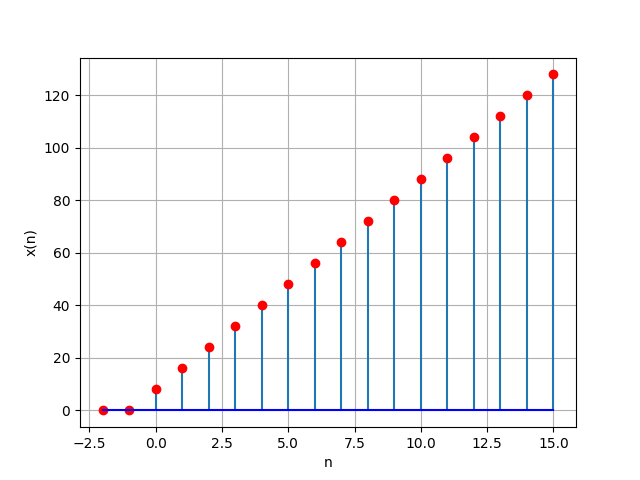
\includegraphics[width=\columnwidth]{figs/a.png}
        \caption{Plot of x(n) $vs$ n}
        \label{fig:1}
    \end{figure}
\begin{align}
    u\brak{n} \system{Z} U\brak{x}
\end{align}
\begin{align}
    U(z) &= \sum\limits_{n=-\infty}^{\infty}z^{-n}u(n)  \\
    U(z) &= \sum\limits_{n=0}^{\infty}z^{-n}   \\
    &= {(1-{z}^{-1})}^{-1} \, ;\, ROC=|z|>1  \\
    \dfrac{d(U(z))}{dz} &= \sum\limits_{n=0}^{\infty}-nz^{-n-1}   \\
    &=-{z}^{-2} {(1-{z^{-1}})}^{-2} \, ; \, ROC:|z|>1
\end{align}
Now,
\begin{align}
    x\brak{n} \system{Z} X\brak{x}
\end{align}
\begin{align}
    X\brak{z} &= \sum\limits_{n=-\infty}^{\infty}x\brak{n} z^{-n}   \\
\end{align}
\begin{align}
   \boxed{ x\brak{n}=\brak{8+8n} \times u\brak{n} } 
\end{align}
\begin{align}
    X(z )&= \sum\limits_{n=-\infty}^{\infty} 8\brak{n+1} \cdot u\brak{n} z^{-n}  \\
    &= \sum\limits_{n=0}^{\infty} 8\brak{n+1} z^{-n}    \\
    &= 8U(n)+8\left (-z\dfrac{d(U(z))}{dz}\right )   \\
    &= 8{(1-{z}^{-1})}^{-1}+8{z}^{-1} {(1-{z^{-1}})}^{-2} \, ; \, ROC:|z|>1 
\end{align}
\begin{table}[htbp]
    \centering
    \def\arraystretch{1.5}
    \begin{tabular}{|p{2.3cm}|p{2.3cm}|p{2.3cm}|}
    \hline
    PARAMETER & VALUE & DESCRIPTION  \\ \hline
    x(n) & \brak{8+8n} & General term of the series  \\ \hline
    X(n) & $8z{(z-1)}^{-1}+8z{(z-1)}^{-2}$ & Z-transform of x(n)  \\ \hline
    u(n) & & Unit step function \\ \hline
    U(n) & $z{(z-1)}^{-1}$ & Z-transform of u(n) \\ \hline
  \end{tabular}
    \caption{Parameter Table2}
    \label{tab:2}
\end{table}

\end{document}
